\documentclass[12pt]{article}
\usepackage{caption}
\usepackage{graphicx, subfig}
\usepackage{float}
\usepackage{mathptmx}
\usepackage{graphicx}
\usepackage{listings}
\usepackage{amsmath}
\usepackage{amssymb}
\usepackage{algorithm}
\usepackage{color}

\definecolor{dkgreen}{rgb}{0,0.6,0}
\definecolor{gray}{rgb}{0.5,0.5,0.5}
\definecolor{mauve}{rgb}{0.58,0,0.82}

\lstset{frame=tb,
  language=Python,
  aboveskip=3mm,
  belowskip=3mm,
  showstringspaces=false,
  columns=flexible,
  basicstyle={\small\ttfamily},
  numbers=none,
  numberstyle=\tiny\color{gray},
  keywordstyle=\color{blue},
  commentstyle=\color{dkgreen},
  stringstyle=\color{mauve},
  breaklines=true,
  breakatwhitespace=true,
  tabsize=3
}
\title{Exploration 3}
\author{Student Name: Fanjie Kong
\\
Student ID: 2462691 }

\begin{document}
\maketitle
\newpage
\textbf{Part 1} : Using the parameters of the Low Threshold Spiking (LTS) Izhikevich model
(a=0.02, b=0.25, c=-65.0, d=2) http://www.izhikevich.org/publications/spikes.htm,
develop a model of three neurons. All three neurons should have their own controllable
input currents. You can use three different TimedArrays or manage the currents through a
series of run commands. Use the basic alpha conductance ,g, to connect the neurons with
the equations
 
$$ g= dg/dt =
−g/\tau_{syn}
+z(t)$$
 
$$ z= dz/dt =
−z/tau_{syn}
+g_{syn}u(t)$$

Modify the code LIFwSynSimp.py where all
the neurons are in a single group to complete the following. 
\\

1. Connect neuron 0 to neuron 1 and neuron 1 to neuron 2 with excitatory
connections with a synaptic time constant of 5ms and a reversal potential of 0.
Establish a steady state with no input current to any neurons for 200 ms. Apply a
suprathreshold stimulus for 20ms neuron 0. Show how the response changes in
neurons 1 and 2 as you change $g_{peak}$ from 0.01 to 0.08.
\\

\textbf{Answer:} 
\\

The color of neuron 0, 1 ,2 are green, red and blue. And the first curve of each neuron is the curve of v, and the second curve is the curve of g(The conductance represents the ion current caused by post-synaptic spikes.).

As the $g_{peak}$ increases, the post-synaptic spikes become more dense, due to increasing synaptic current caused by growing conductance of alpha synapse equation.

 \begin{figure}[H]
  \centering
  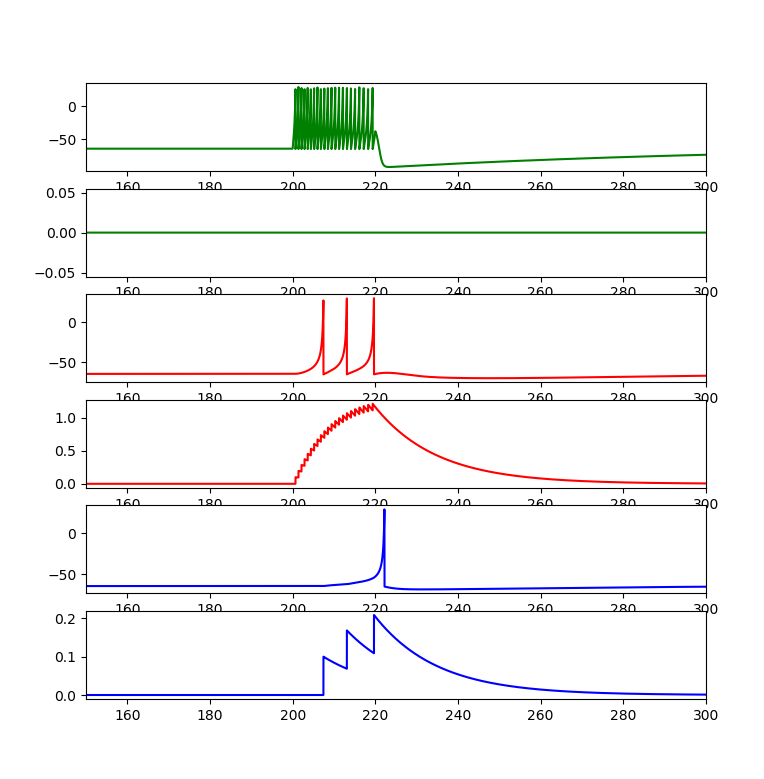
\includegraphics[width=.8\textwidth]{h1_p1_001.png} %1.png是图片文件的相对路径
  \label{img} %此处的label相当于一个图片的专属标志,目的是方便上下文的引用
  \caption{Result $g_{peak}=0.01$}
\end{figure}

 \begin{figure}[H]
  \centering
  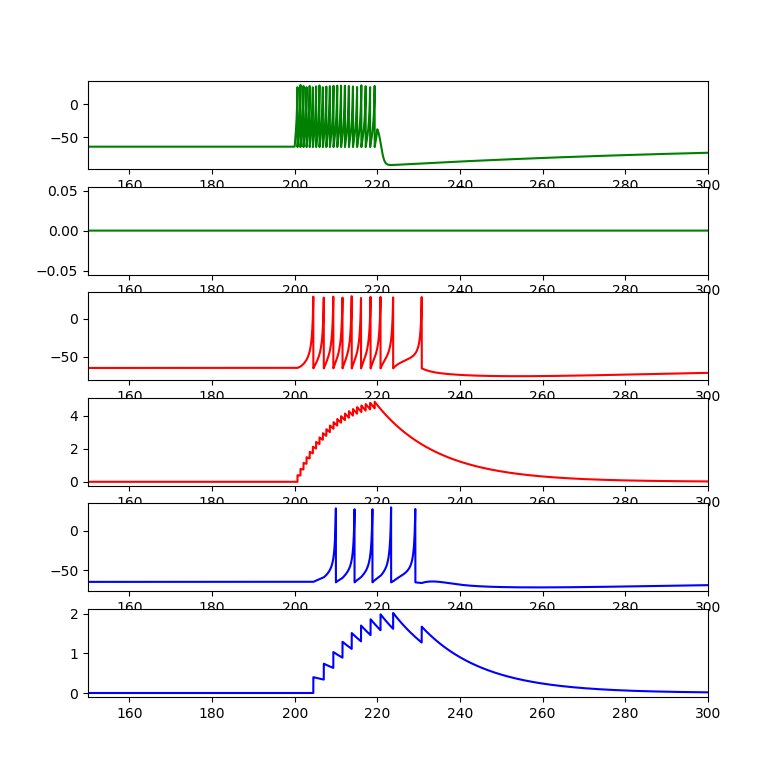
\includegraphics[width=.8\textwidth]{h3_p1_p1_004.png} %1.png是图片文件的相对路径
  \label{img} %此处的label相当于一个图片的专属标志,目的是方便上下文的引用
  \caption{Result $g_{peak}=0.04$}
\end{figure}
  \begin{figure}[H]
  \centering
  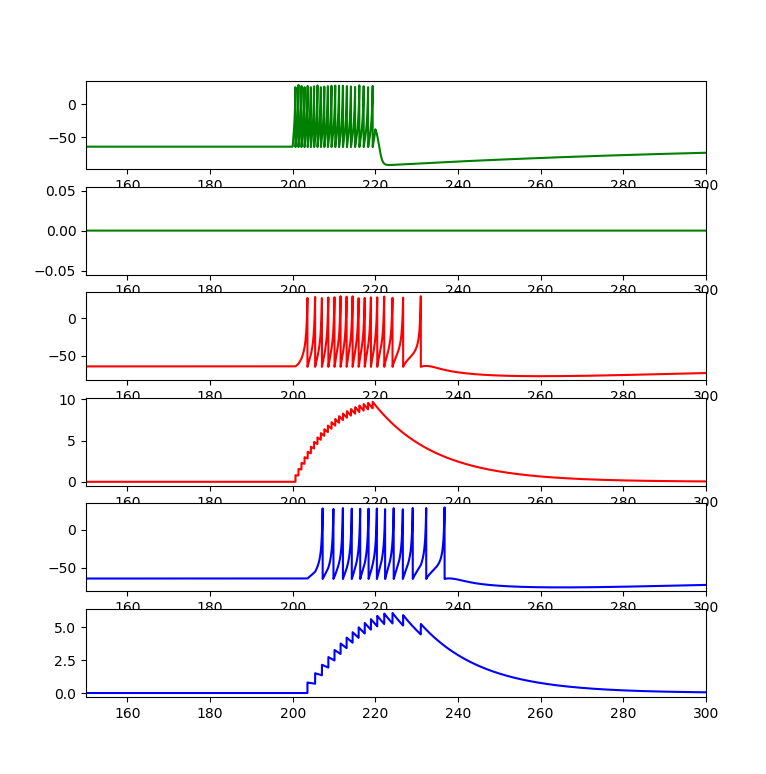
\includegraphics[width=.8\textwidth]{h3_p1_p1_008.png} %1.png是图片文件的相对路径
  \label{img} %此处的label相当于一个图片的专属标志,目的是方便上下文的引用
  \caption{Result $g_{peak}=0.08$}
\end{figure}
 \begin{figure}[H]
  \centering
  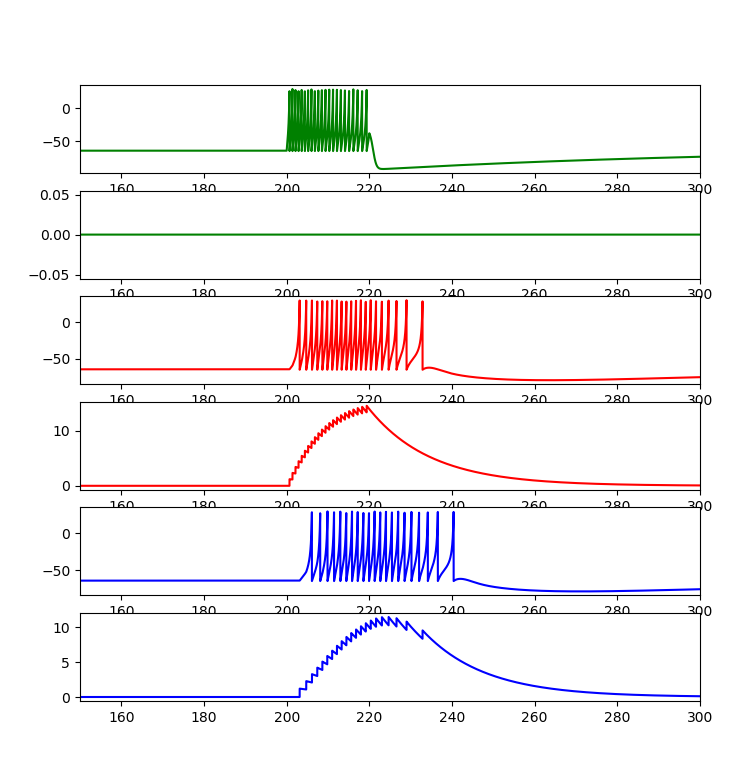
\includegraphics[width=.8\textwidth]{h3_p1_p1_012.png} %1.png是图片文件的相对路径
  \label{img} %此处的label相当于一个图片的专属标志,目的是方便上下文的引用
  \caption{Result $g_{peak}=0.12$}
\end{figure}
\newpage

2. Incorporate synaptic delays to the case above of 5ms. How does the response change?
\\

\textbf{Answer:} 
\\

The conductance and voltage response of neuron 1 and 2 will be delayed. The response of neuron 2 will be delayed twice as much as delay time.
\begin{figure}[H]
  \centering
  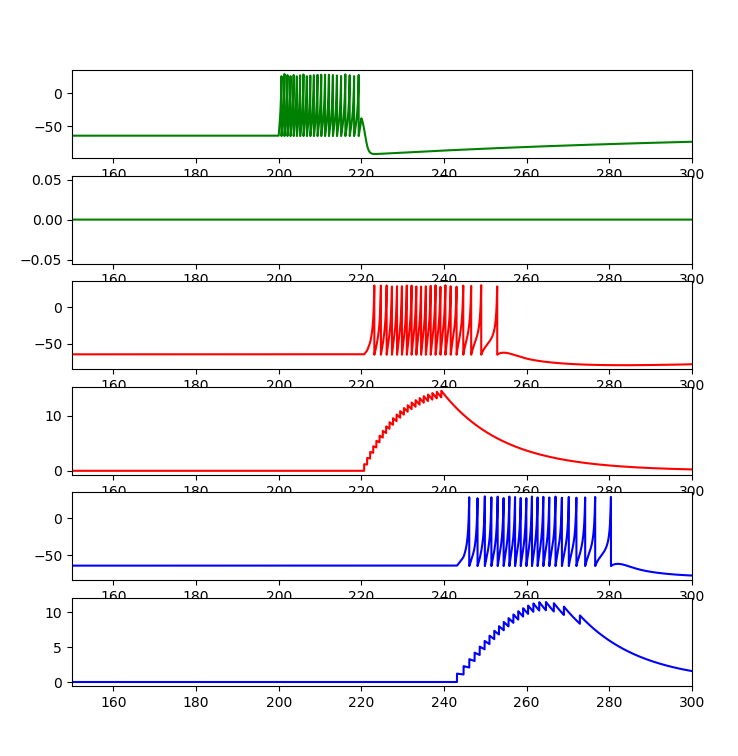
\includegraphics[width=.8\textwidth]{h3_p1_p2.png} %1.png是图片文件的相对路径
  \label{img} %此处的label相当于一个图片的专属标志,目的是方便上下文的引用
  \caption{Result $delay time = 20 ms$}
\end{figure}

\newpage

3. Connect neuron 0 to neuron 1 with inhibitory connections with a synaptic time
constant of 5ms and a reversal potential of -80. Do not connect any cell to neuron
2. Reach steady state at 200ms with no stimulus and apply the same
suprathreshold input currents to each cell. Here neuron 0 and 2 should generate
the same response. What happens to neuron 1 as $g_{peak}$ is varied from 0.02 to 0.12
\\

\textbf{Answer:} 
\\

The voltage response of neuron 1 will be inhibited by the synaptic current. As the $g_{peak}$ increases, the influence becomes more obvious due to higher inhibitory synaptic current. And the spikes of neuron 1 becomes more sparse as the $g_{peak}$ grows.

\begin{figure}[H]
  \centering
  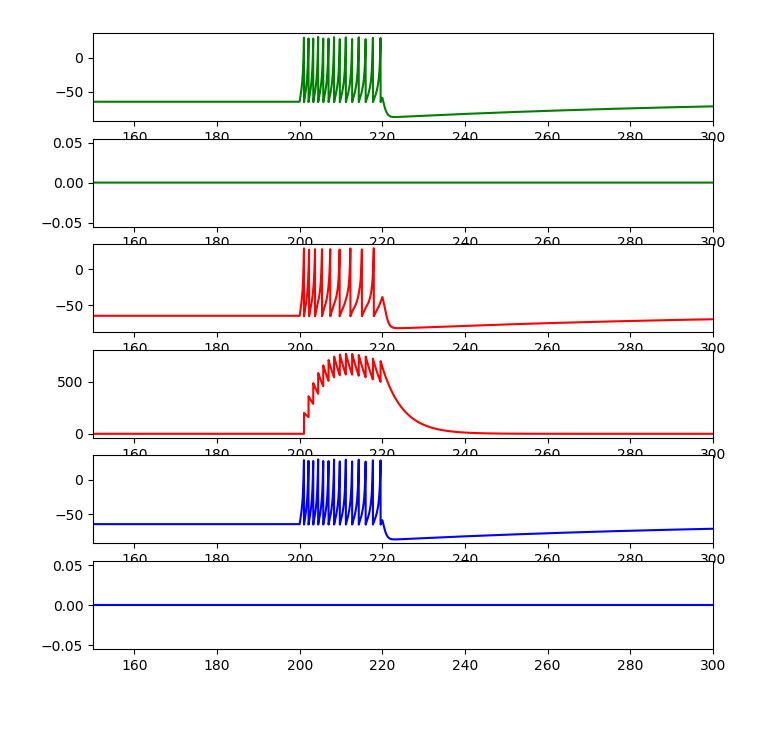
\includegraphics[width=.8\textwidth]{h3_p1_p3_200.png} %1.png是图片文件的相对路径
  \label{img} %此处的label相当于一个图片的专属标志,目的是方便上下文的引用
  \caption{Result $g_{peak} = 0.02 $}
\end{figure}
\begin{figure}[H]
  \centering
  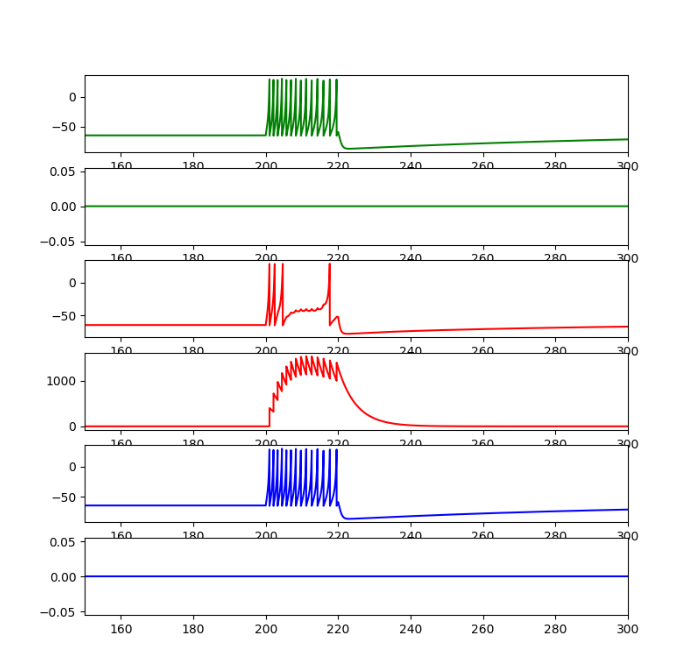
\includegraphics[width=.8\textwidth]{h3_p1_p3_400.png} %1.png是图片文件的相对路径
  \label{img} %此处的label相当于一个图片的专属标志,目的是方便上下文的引用
  \caption{Result $g_{peak} = 0.04 $}
\end{figure}
\begin{figure}[H]
  \centering
  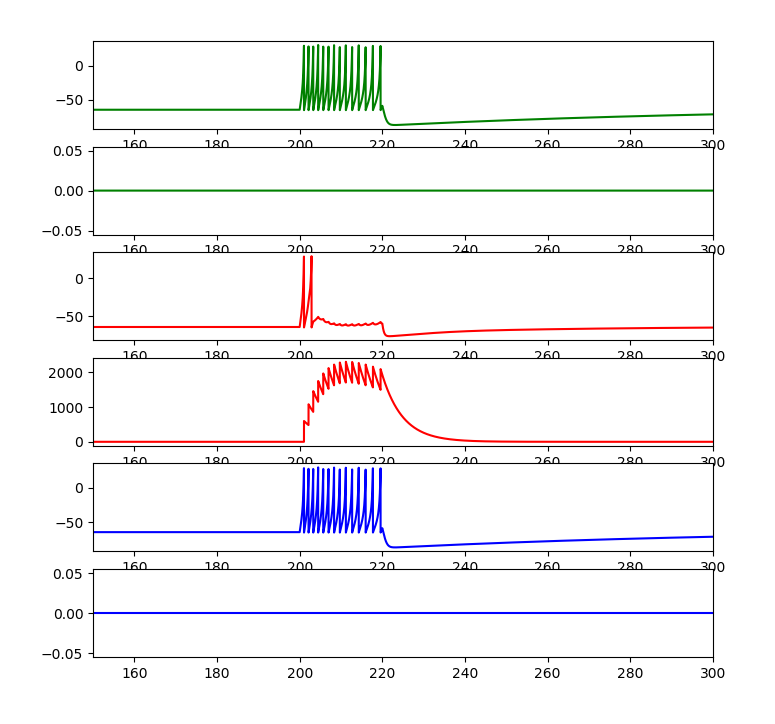
\includegraphics[width=.8\textwidth]{h3_p1_p3_600.png} %1.png是图片文件的相对路径
  \label{img} %此处的label相当于一个图片的专属标志,目的是方便上下文的引用
  \caption{Result $g_{peak} = 0.06 $}
\end{figure}
\begin{figure}[H]
  \centering
  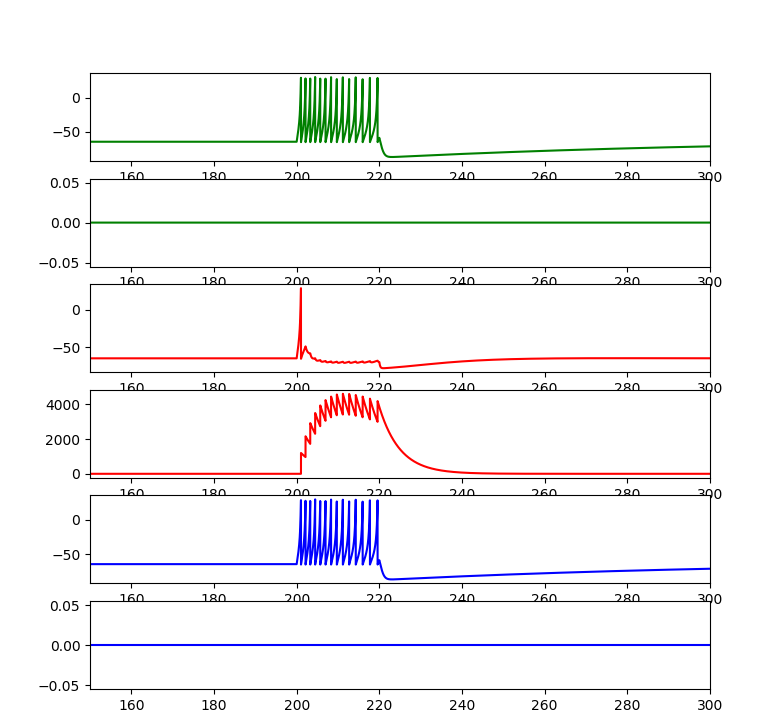
\includegraphics[width=.8\textwidth]{h3_p1_p3_1200.png} %1.png是图片文件的相对路径
  \label{img} %此处的label相当于一个图片的专属标志,目的是方便上下文的引用
  \caption{Result $g_{peak} = 0.12 $}
\end{figure}
\newpage

4. Incorporate synaptic delays to the case above of 5ms. How does the response change?
\\

\textbf{Answer:} 
\\

The inhibitory impact on neuron 1 will be delayed due to the delay of synaptic current.
\begin{figure}[H]
  \centering
  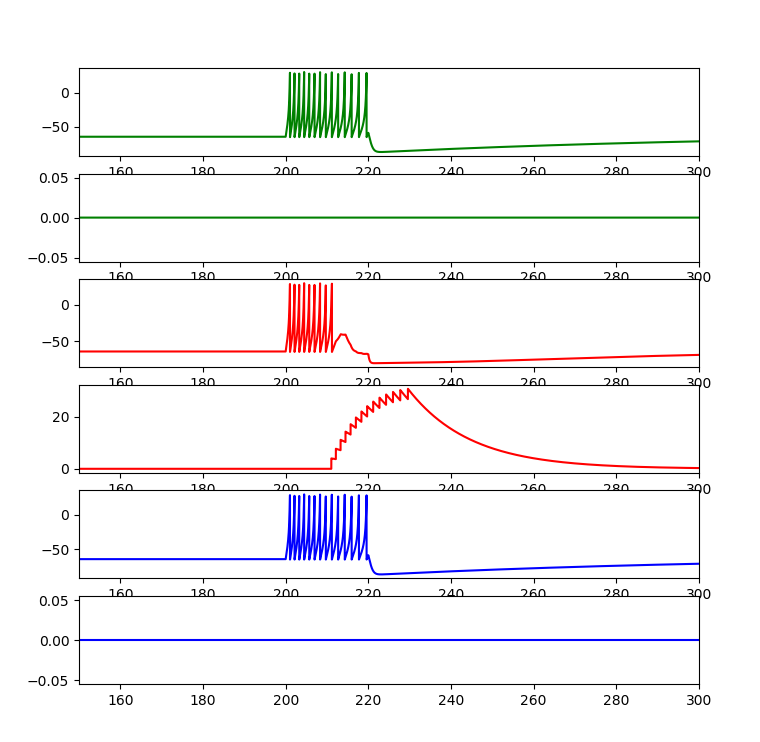
\includegraphics[width=.8\textwidth]{h3_p1_p3_delay.png} %1.png是图片文件的相对路径
  \label{img} %此处的label相当于一个图片的专属标志,目的是方便上下文的引用
  \caption{Result $delay time = 10 ms$}
\end{figure}
\newpage

5. Design several interesting circuits using excitatory AND inhibitory connections
with 4 neurons. Note that one cell type should be able to produce only one type of
synapse (inhibitory or excitatory) but a cell can receive both types. Explain the
output based on your design.
\\

\textbf{Answer:} 
\\

The connection of neuron 0 and 1 is excitatory. The connection of neuron 1 and 2 is inhibitory.
The connection of neuron 2 and 3 is excitatory.

Now I apply the suprathreshold current on neuron 0 and neuron 2. The outcome is that the spikes of neuron 2 will be inhibited by the influence of neuron 0 and 1, thus inhibiting the spikes of neuron 3.

And then I cancel the current on neuron 0. Neuron 2 can generate spikes without obstacle to stimulate neuron 3.

And I find the interesting phenomenon that there is a spike after the inhibitory influence. I think it is because low 'v' causes low 'u' according to $du/dt = a(bv-u)$. Thus in this situation, the neuron is easy to fire.
\begin{figure}[H]
  \centering
  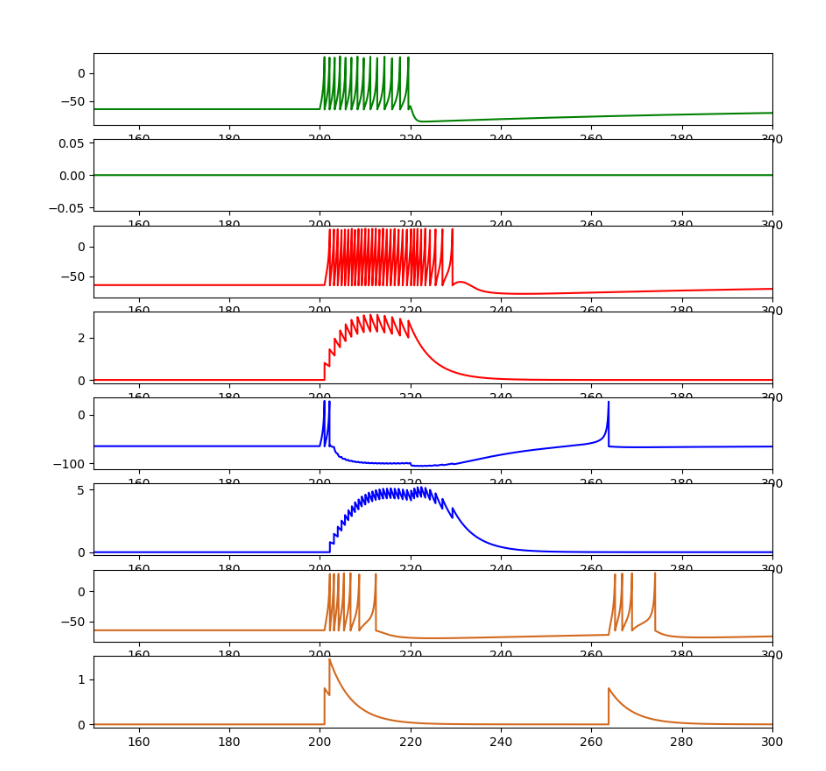
\includegraphics[width=.8\textwidth]{h3_p1_p5_1.png} %1.png是图片文件的相对路径
  \label{img} %此处的label相当于一个图片的专属标志,目的是方便上下文的引用
  \caption{Apply current to neuron 0 and 2 }
\end{figure}
\begin{figure}[H]
  \centering
  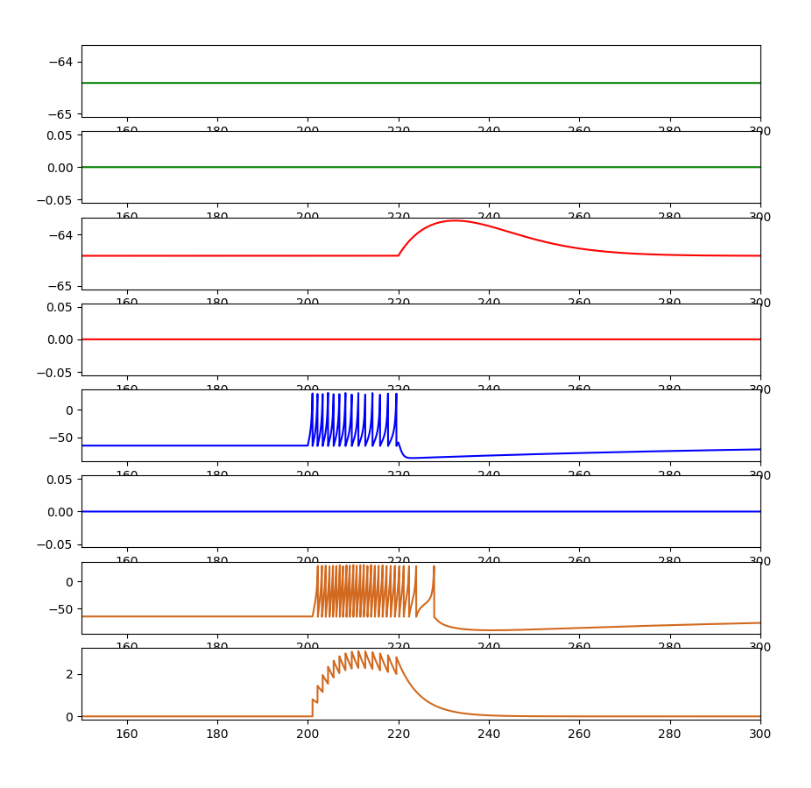
\includegraphics[width=.8\textwidth]{h3_p1_p5_2.png} %1.png是图片文件的相对路径
  \label{img} %此处的label相当于一个图片的专属标志,目的是方便上下文的引用
  \caption{Apply current just to neuron 2 }
\end{figure}

\newpage
\textbf{Part 2}
\\

Use the framework of synaptic connections to form a network of 4 neurons to
actuate the bug as a coward. Modify LIFwSynSimp two have 4 different groups with 1
neuron in each group.  Find synapatic conductances that give you a large dynamic range.  
\\

\textbf{Answer:} 
\\

The value of synaptic conductance will have impact on the post-synaptic spikes. As the synaptic conductance increases, the post-synaptic spikes become more dense. However, when the conductance it excessively high like 0.2, the membrane potential of post-synaptic will keep depolarization and there are no spikes during this time.

When the synaptic conductance is about 0.12, it will have the large dynamic range as shown in figure.

What is more, The meaning of the parameters I find is that the magnitude of velocity is directly dependent on the parameter $\eta$. $\tau_{motor}$ can control the decay rate of the velocity.
\begin{figure}[H]
\centering
    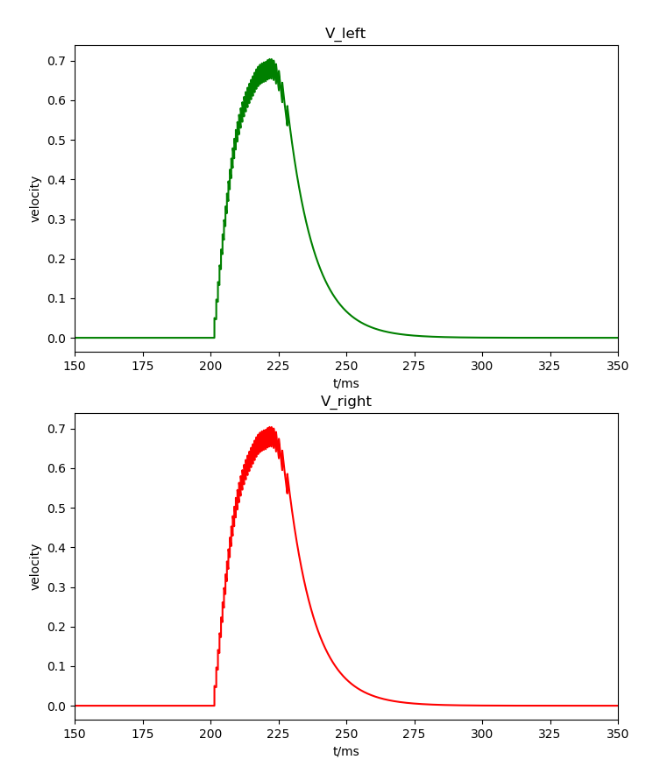
\includegraphics[width=.8\textwidth]{h3_p2_1000.png} %1.png是图片文件的相对路径
  \label{img} %此处的label相当于一个图片的专属标志,目的是方便上下文的引用
  \caption{The large dynamic range of velocity when $g_{peak} = 0.12$}
\end{figure}

 \begin{figure}[H]
  \centering
    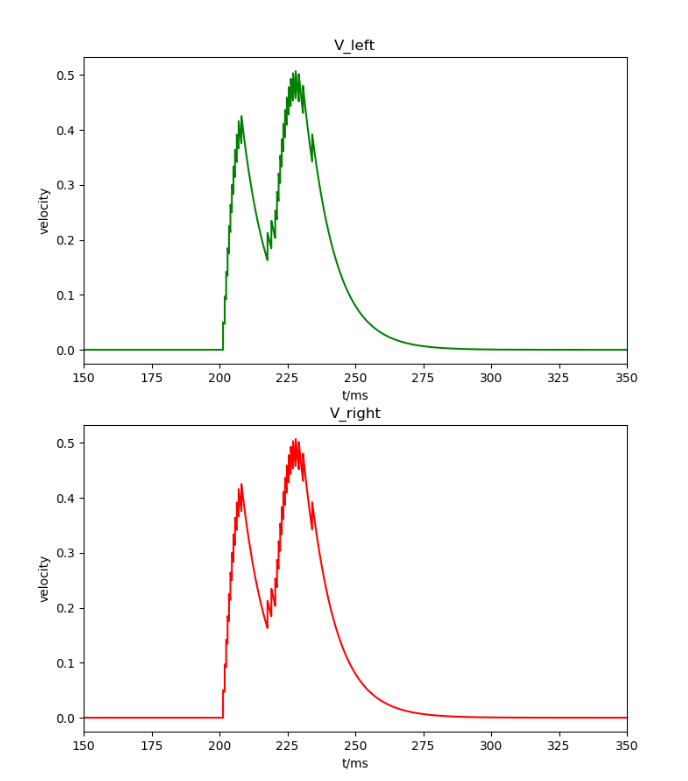
\includegraphics[width=.8\textwidth]{h3_p2_1500.png} %1.png是图片文件的相对路径
  \caption{$g_{peak}=0.2$ }
\end{figure}

\begin{figure}
\centering
      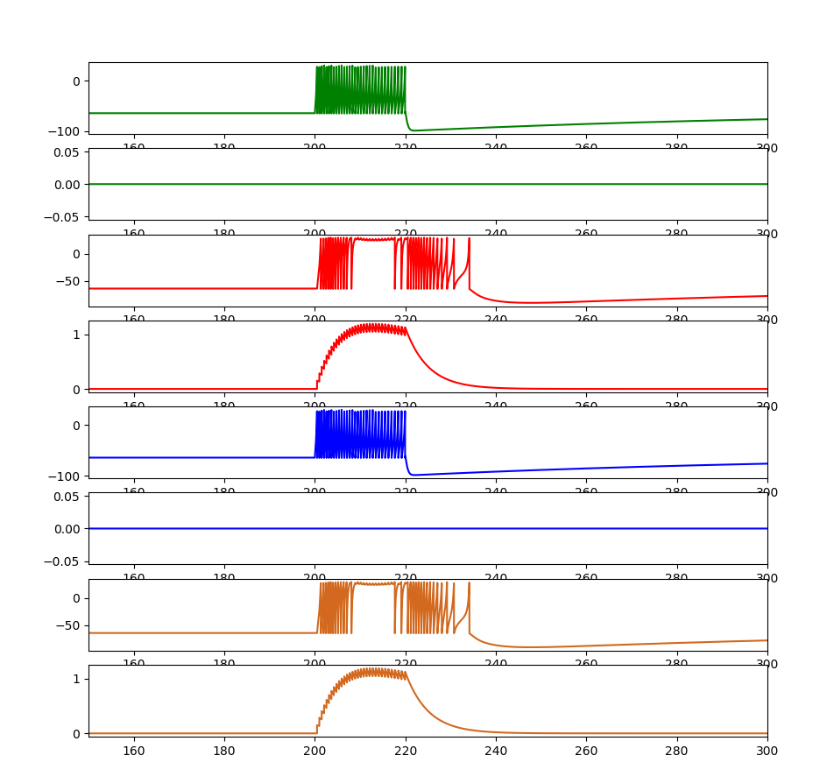
\includegraphics[width=.8\textwidth]{h3_p2_c.png} %1.png是图片文件的相对路径
       \caption{The membrane potential of neuron and post-synaptic conductance when $g_{peak}=0.2$ }
  \label{img} %此处的label相当于一个图片的专属标志,目的是方便上下文的引用
\end{figure}

\newpage
\large \textbf{Appendix}
\\

\normalsize\textbf{Part1 problem 1 \& problem 2}
\\

\lstset{language=Python}
\begin{lstlisting}
from brian2 import *
defaultclock.dt=.01*ms
num_neurons = 2
duration = 2*second

# Parameters
area = 20000*umetre**2
Cm = 1*ufarad*cm**-2
El = -60*mV
gl = 0.7*msiemens/cm**2

tau_ampa=0.3*ms
g_synpk= 120 * siemens
g_synmaxval=(g_synpk)
E_syn = 0*mV
tau_m = 15*ms
# Parameters for LTS model
a = 0.02
b = 0.25
c = -65*mV
d = 2.0 * mV
R = 1*ohm
v0 = -65*mV
u0 = 4*mV

#The model
eqs_fv = '''
fv = 0.04*v**2 / mV + 5*v + 140*mV : volt
 '''
eqs_u = '''
du/dt = a*(b*v - u) * metre ** 2 * kilogram * second ** -4 * amp ** -1 /mV: volt
'''
eqs = '''
dv/dt = ((fv - u + R*I)* metre ** 2 * kilogram * second ** -4 * amp ** -1 /mV) + (g*(E_syn-v)*metre ** 2 * kilogram * second ** -4 * amp ** -1/amp) : volt
I : amp
'''
eqs_syn = '''
# The conductance of the alpha model
dz/dt = (-z/tau_m) : siemens
dg/dt = -g/tau_m + z/ms : siemens
'''

eqs += eqs_fv + eqs_u + eqs_syn
# Threshold and refractoriness are only used for spike counting
neuron1 = NeuronGroup(1, eqs,
                    threshold='v >= 30*mV',
                    reset='v = c;u = u + d',
                    method='euler',
                    refractory='v > 0*mV')
neuron2 = NeuronGroup(1, eqs,
                    threshold='v >= 30*mV',
                    reset='v = c;u = u + d',
                    method='euler',
                    refractory='v > 0*mV'
                      )
neuron3 = NeuronGroup(1, eqs,
                    threshold='v >= 30*mV',
                    reset='v = c;u = u + d',
                    method='euler',
                    refractory='v > 0*mV'
                      )

syn1 = Synapses(neuron1, neuron2, clock=neuron1.clock, on_pre='''g += g_synpk''')
syn2 = Synapses(neuron2, neuron3, clock=neuron2.clock, on_pre='''g += g_synpk''')
syn1.connect('i == j')
syn2.connect('i == j')
syn1.delay=20*ms
syn2.delay=20*ms

monitor1=StateMonitor(neuron1, ('v', 'g'), record=True)
monitor2=StateMonitor(neuron2, ('v', 'g'), record=True)
monitor3=StateMonitor(neuron3, ('v', 'g'), record=True)
neuron1.v= -65*mV
neuron1.u= b*(-65*mV)
neuron2.v= -65*mV
neuron2.u= b*(-65*mV)
neuron3.v= -65*mV
neuron3.u= b*(-65*mV)

neuron1.g= 0*nsiemens
neuron2.g = 0*nsiemens
neuron3.g = 0*nsiemens
run(200.0*ms, report='text')
neuron1.I = 75*mA
neuron2.I = 0*nA
neuron3.I = 0*nA
run(20.0*ms, report='text')
neuron1.I = 0*mA
neuron2.I = 0*nA
neuron3.I = 0*nA
run(400.0*ms, report='text')


figure(1, figsize=(8, 8))
subplot(6, 1, 1)
plot(monitor1.t/ms, monitor1.v[0]/mV, 'g')
xlim(150, 300)
subplot(6, 1, 2)
plot(monitor1.t/ms, monitor1.g[0], 'g')
xlim(150, 300)
subplot(6, 1, 3)
plot(monitor2.t/ms, monitor2.v[0]/mV, 'r')
xlim(150, 300)
subplot(6, 1, 4)
plot(monitor2.t/ms, monitor2.g[0]/100, 'r')
xlim(150, 300)
subplot(6, 1, 5)
plot(monitor3.t/ms, monitor3.v[0]/mV, 'b')
xlim(150, 300)
subplot(6, 1, 6)
plot(monitor3.t/ms, monitor3.g[0]/100, 'b')
xlim(150, 300)
show()
\end{lstlisting}
\newpage
\normalsize\textbf{Part1 problem 3 \& problem 4}
\\

\lstset{language=Python}
\begin{lstlisting}
from brian2 import *
defaultclock.dt=.01*ms
num_neurons = 2
duration = 2*second

# Parameters
area = 20000*umetre**2
Cm = 1*ufarad*cm**-2
El = -60*mV
gl = 0.7*msiemens/cm**2

tau_ampa=0.3*ms
g_synpk= 400 * siemens
g_synmaxval=(g_synpk)
E_syn = -80*mV
tau_m = 15*ms
# Parameters for LTS model
a = 0.02
b = 0.25
c = -65*mV
d = 2.0 * mV
R = 1*ohm
v0 = -65*mV
u0 = 4*mV

#The model
eqs_fv = '''
fv = 0.04*v**2 / mV + 5*v + 140*mV : volt
 '''
eqs_u = '''
du/dt = a*(b*v - u) * metre ** 2 * kilogram * second ** -4 * amp ** -1 /mV: volt
'''
eqs = '''
dv/dt = ((fv - u + R*I)* metre ** 2 * kilogram * second ** -4 * amp ** -1 /mV) + (g*(E_syn-v)*metre ** 2 * kilogram * second ** -4 * amp ** -1/amp) : volt
I : amp
'''
eqs_syn = '''
# The conductance of the alpha model
dz/dt = (-z/tau_m) : siemens
dg/dt = -g/tau_m + z/ms : siemens
'''

eqs += eqs_fv + eqs_u + eqs_syn
# Threshold and refractoriness are only used for spike counting
neuron1 = NeuronGroup(1, eqs,
                    threshold='v >= 30*mV',
                    reset='v = c;u = u + d',
                    method='euler'
                    )
neuron2 = NeuronGroup(1, eqs,
                    threshold='v >= 30*mV',
                    reset='v = c;u = u + d',
                    method='euler'
                      )
neuron3 = NeuronGroup(1, eqs,
                    threshold='v >= 30*mV',
                    reset='v = c;u = u + d',
                    method='euler'
                      )
neuron4 = NeuronGroup(1, eqs,
                    threshold='v >= 30*mV',
                    reset='v = c;u = u + d',
                    method='euler'
                      )
syn1 = Synapses(neuron1, neuron2, clock=neuron1.clock, on_pre='''g += g_synpk''')
# syn2 = Synapses(neuron2, neuron3, clock=neuron2.clock, on_pre='''g += g_synpk''')
syn1.connect('i == j')
syn1.delay=10*ms
# syn2.delay=15*ms

monitor1=StateMonitor(neuron1, ('v', 'g'), record=True)
monitor2=StateMonitor(neuron2, ('v', 'g'), record=True)
monitor3=StateMonitor(neuron3, ('v', 'g'), record=True)
monitor4=StateMonitor(neuron4, ('v', 'g'), record=True)

neuron1.v= -65*mV
neuron1.u= b*(-65*mV)
neuron2.v= -65*mV
neuron2.u= b*(-65*mV)
neuron3.v= -65*mV
neuron3.u= b*(-65*mV)
neuron4.v= -65*mV
neuron4.u= b*(-65*mV)


neuron1.g= 0*nsiemens
neuron2.g = 0*nsiemens
neuron3.g = 0*nsiemens
run(200.0*ms, report='text')
neuron1.I = 40*mA
neuron2.I = 40*mA
neuron3.I = 40*mA
run(20.0*ms, report='text')
neuron1.I = 0*mA
neuron2.I = 0*nA
neuron3.I = 0*nA
run(200.0*ms, report='text')


figure(1, figsize=(8, 8))
subplot(6, 1, 1)
plot(monitor1.t/ms, monitor1.v[0]/mV, 'g')
xlim(150, 300)
subplot(6, 1, 2)
plot(monitor1.t/ms, monitor1.g[0], 'g')
xlim(150, 300)
subplot(6, 1, 3)
plot(monitor2.t/ms, monitor2.v[0]/mV, 'r')
xlim(150, 300)
subplot(6, 1, 4)
plot(monitor2.t/ms, monitor2.g[0]/100, 'r')
xlim(150, 300)
subplot(6, 1, 5)
plot(monitor3.t/ms, monitor3.v[0]/mV, 'b')
xlim(150, 300)
subplot(6, 1, 6)
plot(monitor3.t/ms, monitor3.g[0]/100, 'b')
xlim(150, 300)
show()
\end{lstlisting}
\newpage

\normalsize\textbf{Part1 problem 5}
\\

\lstset{language=Python}
\begin{lstlisting}
from brian2 import *
defaultclock.dt=.01*ms
num_neurons = 2
duration = 2*second

# Parameters
area = 20000*umetre**2
Cm = 1*ufarad*cm**-2
El = -60*mV
gl = 0.7*msiemens/cm**2

tau_ampa=0.3*ms
g_synpk= 800 * siemens
g_synmaxval=(g_synpk)
E_syn_in = -80*mV
E_syn_ex = 0*mV
tau_m = 5*ms
# Parameters for LTS model
a = 0.02
b = 0.25
c = -65*mV
d = 2.0 * mV
R = 1*ohm
v0 = -65*mV
u0 = 4*mV

#The model
eqs_fv = '''
fv = 0.04*v**2 / mV + 5*v + 140*mV : volt
 '''
eqs_u = '''
du/dt = a*(b*v - u) * metre ** 2 * kilogram * second ** -4 * amp ** -1 /mV: volt
'''
eqs = '''
dv/dt = ((fv - u + R*I)* metre ** 2 * kilogram * second ** -4 * amp ** -1 /mV) + (g*(E_syn-v)*metre ** 2 * kilogram * second ** -4 * amp ** -1/amp) : volt
I : amp
E_syn : volt 
'''
eqs_syn = '''
# The conductance of the alpha model
dz/dt = (-z/tau_m) : siemens
dg/dt = -g/tau_m + z/ms : siemens
'''

eqs += eqs_fv + eqs_u + eqs_syn
# Threshold and refractoriness are only used for spike counting
neuron1 = NeuronGroup(1, eqs,
                    threshold='v >= 30*mV',
                    reset='v = c;u = u + d',
                    method='euler'
                    )
neuron2 = NeuronGroup(1, eqs,
                    threshold='v >= 30*mV',
                    reset='v = c;u = u + d',
                    method='euler'
                      )
neuron3 = NeuronGroup(1, eqs,
                    threshold='v >= 30*mV',
                    reset='v = c;u = u + d',
                    method='euler'
                      )
neuron4 = NeuronGroup(1, eqs,
                    threshold='v >= 30*mV',
                    reset='v = c;u = u + d',
                    method='euler'
                      )
syn1 = Synapses(neuron1, neuron2, clock=neuron1.clock, on_pre='''g += g_synpk''')
syn2 = Synapses(neuron2, neuron3, clock=neuron2.clock, on_pre='''g += g_synpk''')
syn3 = Synapses(neuron3, neuron4, clock=neuron2.clock, on_pre='''g += g_synpk''')

syn1.connect('i == j')
syn2.connect('i == j')
syn3.connect('i == j')
# syn1.delay=10*ms
# syn2.delay=20*ms
syn3.delay = 0*ms

monitor1=StateMonitor(neuron1, ('v', 'g'), record=True)
monitor2=StateMonitor(neuron2, ('v', 'g'), record=True)
monitor3=StateMonitor(neuron3, ('v', 'g'), record=True)
monitor4=StateMonitor(neuron4, ('v', 'g'), record=True)

neuron1.v= -65*mV
neuron1.u= b*(-65*mV)
neuron2.v= -65*mV
neuron2.u= b*(-65*mV)
neuron3.v= -65*mV
neuron3.u= b*(-65*mV)
neuron4.v= -65*mV
neuron4.u= b*(-65*mV)


neuron1.g= 0*nsiemens
neuron2.g = 0*nsiemens
neuron3.g = 0*nsiemens
neuron4.g = 0*nsiemens

run(200.0*ms, report='text')
# Define the type of neuron
neuron1.E_syn = E_syn_ex
neuron2.E_syn = E_syn_ex
neuron3.E_syn = 1.5 * E_syn_in
neuron4.E_syn = E_syn_ex

neuron1.I = 0*mA
neuron2.I = 0*mA
neuron3.I = 40*mA
neuron4.I = 0*mA
run(20.0*ms, report='text')
neuron2.u= b*(-65*mV)
neuron1.I = 0*mA
neuron2.I = 0*nA
neuron3.I = 0*nA
neuron4.I = 0*mA
run(200.0*ms, report='text')


figure(1, figsize=(10, 10))
subplot(8, 1, 1)
plot(monitor1.t/ms, monitor1.v[0]/mV, 'g')
xlim(150, 300)
subplot(8, 1, 2)
plot(monitor1.t/ms, monitor1.g[0]/1000, 'g')
xlim(150, 300)
subplot(8, 1, 3)
plot(monitor2.t/ms, monitor2.v[0]/mV, 'r')
xlim(150, 300)
subplot(8, 1, 4)
plot(monitor2.t/ms, monitor2.g[0]/1000, 'r')
xlim(150, 300)
subplot(8, 1, 5)
plot(monitor3.t/ms, monitor3.v[0]/mV, 'b')
xlim(150, 300)
subplot(8, 1, 6)
plot(monitor3.t/ms, monitor3.g[0]/1000, 'b')
xlim(150, 300)
subplot(8, 1, 7)
plot(monitor4.t/ms, monitor4.v[0]/mV, 'chocolate')
xlim(150, 300)
subplot(8, 1, 8)
plot(monitor4.t/ms, monitor4.g[0]/1000, 'chocolate')
xlim(150, 300)
show()

\end{lstlisting}
\newpage
\normalsize\textbf{Part2 }
\\

\lstset{language=Python}
\begin{lstlisting}
from brian2 import *
defaultclock.dt=.01*ms
num_neurons = 2
duration = 2*second

# Parameters
area = 20000*umetre**2
Cm = 1*ufarad*cm**-2
El = -60*mV
gl = 0.7*msiemens/cm**2

tau_ampa=0.3*ms
g_synpk= 1500 * siemens
g_synmaxval=(g_synpk)
E_syn_in = -80*mV
E_syn_ex = 0*mV
tau_m = 5*ms
# Parameters for LTS model
a = 0.02
b = 0.25
c = -65*mV
d = 2.0 * mV
R = 1*ohm
v0 = -65*mV
u0 = 4*mV
# parameters for motor
tau_motor = 10*ms
eta = 0.05
#The model
eqs_fv = '''
fv = 0.04*v**2 / mV + 5*v + 140*mV : volt
 '''
eqs_u = '''
du/dt = a*(b*v - u) * metre ** 2 * kilogram * second ** -4 * amp ** -1 /mV: volt
'''
eqs = '''
dv/dt = ((fv - u + R*I)* metre ** 2 * kilogram * second ** -4 * amp ** -1 /mV) + (g*(E_syn-v)*metre ** 2 * kilogram * second ** -4 * amp ** -1/amp) : volt
I : amp
E_syn : volt 
'''
eqs_syn = '''
# The conductance of the alpha model
dz/dt = (-z/tau_m) : siemens
dg/dt = -g/tau_m + z/ms : siemens
'''

eqs += eqs_fv + eqs_u + eqs_syn
# Threshold and refractoriness are only used for spike counting
neuron1 = NeuronGroup(1, eqs,
                    threshold='v >= 30*mV',
                    reset='v = c;u = u + d',
                    method='euler'
                    )
neuron2 = NeuronGroup(1, eqs,
                    threshold='v >= 30*mV',
                    reset='v = c;u = u + d',
                    method='euler'
                      )
neuron3 = NeuronGroup(1, eqs,
                    threshold='v >= 30*mV',
                    reset='v = c;u = u + d',
                    method='euler'
                      )
neuron4 = NeuronGroup(1, eqs,
                    threshold='v >= 30*mV',
                    reset='v = c;u = u + d',
                    method='euler'
                      )
neuron_L = NeuronGroup(1, '''
dvl/dt = -(vl/tau_motor) : 1 
''')
neuron_R = NeuronGroup(1, '''
dvr/dt = -(vr/tau_motor) : 1 
''')
syn1 = Synapses(neuron1, neuron2, clock=neuron1.clock, on_pre='''g += g_synpk ''',
                method='euler')

syn2 = Synapses(neuron3, neuron4, clock=neuron3.clock, on_pre='''g += g_synpk''',
                method='euler')
synl = Synapses(neuron2, neuron_L, clock=neuron2.clock, on_pre='''vl += eta''')
synr = Synapses(neuron4, neuron_R, clock=neuron4.clock, on_pre='''vr += eta''')


syn1.connect('i == j')
syn2.connect('i == j')
synl.connect('i == j')
synr.connect('i == j')
# syn1.delay=10*ms
# syn2.delay=20*ms

monitor1=StateMonitor(neuron1, ('v', 'g'), record=True)
monitor2=StateMonitor(neuron2, ('v', 'g'), record=True)
monitor3=StateMonitor(neuron3, ('v', 'g'), record=True)
monitor4=StateMonitor(neuron4, ('v', 'g'), record=True)
monitor_syn1 = StateMonitor(neuron_L, 'vl', record=True)
monitor_syn2 = StateMonitor(neuron_R, 'vr', record=True)

neuron1.v= -65*mV
neuron1.u= b*(-65*mV)
neuron2.v= -65*mV
neuron2.u= b*(-65*mV)
neuron3.v= -65*mV
neuron3.u= b*(-65*mV)
neuron4.v= -65*mV
neuron4.u= b*(-65*mV)


neuron1.g= 0*nsiemens
neuron2.g = 0*nsiemens
neuron3.g = 0*nsiemens
neuron4.g = 0*nsiemens

run(200.0*ms, report='text')
# Define the type of neuron
neuron1.E_syn = E_syn_ex
neuron2.E_syn = E_syn_ex
neuron3.E_syn = E_syn_ex
neuron4.E_syn = E_syn_ex

neuron1.I = 120*mA
neuron2.I = 0*mA
neuron3.I = 120*mA
neuron4.I = 0*mA
run(20.0*ms, report='text')
neuron1.I = 0*mA
neuron2.I = 0*nA
neuron3.I = 0*nA
neuron4.I = 0*mA
run(200.0*ms, report='text')


figure(1, figsize=(8, 10))
subplot(2, 1, 1)
plot(monitor_syn1.t/ms, monitor_syn1.vl[0], 'g')
xlabel('t/ms')
ylabel('velocity')
title("V_left")
xlim(150, 350)
subplot(2, 1, 2)
plot(monitor_syn2.t/ms, monitor_syn2.vr[0], 'r')
xlabel('t/ms')
ylabel('velocity')
title("V_right")
xlim(150, 350)


figure(2, figsize=(10, 10))
subplot(8, 1, 1)
plot(monitor1.t/ms, monitor1.v[0]/mV, 'g')
xlim(150, 300)
subplot(8, 1, 2)
plot(monitor1.t/ms, monitor1.g[0], 'g')
xlim(150, 300)
subplot(8, 1, 3)
plot(monitor2.t/ms, monitor2.v[0]/mV, 'r')
xlim(150, 300)
subplot(8, 1, 4)
plot(monitor2.t/ms, monitor2.g[0]/10000, 'r')
xlim(150, 300)
subplot(8, 1, 5)
plot(monitor3.t/ms, monitor3.v[0]/mV, 'b')
xlim(150, 300)
subplot(8, 1, 6)
plot(monitor3.t/ms, monitor3.g[0], 'b')
xlim(150, 300)
subplot(8, 1, 7)
plot(monitor4.t/ms, monitor4.v[0]/mV, 'chocolate')
xlim(150, 300)
subplot(8, 1, 8)
plot(monitor4.t/ms, monitor4.g[0]/10000, 'chocolate')
xlim(150, 300)
show()
\end{lstlisting}
\end{document}